%% COPYRIGHT: Markus Kollmar
%%
%% This is the main escad manual source. We try document-driven-development.
%% Pictures are stored in "figures" directory and
%% tikz-pictures should be build there before build main escad_manual.tex.
%% We use UTF-8 (UNICODE) encoding for this file and lualatex as latex-engine which works well.
%%
%% BUILD WITH LUALATEX AND FILE UTF-8-ENCODED (RECOMMENDED):
%% lualatex escad_manual.tex
%% biber escad_manual.bcf
%% lualatex escad_manual.tex
%% lualatex escad_manual.tex
%%
%% BUILD WITH PDFLATEX:
%%   pdflatex -interaction=nonstopmode escad_manual.tex
%% BUILD WITH PDFLATEX AND SYNCTEX:
%%   pdflatex -synctex=1 -interaction=nonstopmode escad_manual.tex
%% BUILD WITH EXTERNAL-PACKAGE:
%%   pdflatex -synctex=1 -interaction=nonstopmode --shell-escape escad_manual.tex
%% COMPILATION ALTERNATIVE:
%%   latexmk -pdf escad_manual.tex
%%
%% EMACS STUFF:
%%   (set-keyboard-coding-system 'utf-8)
%%   modes: latex-mode, outline-minor-mode
%%   M-x outline-toggle-children
%%   M-x pdf-tools-install
%%   M-x customize apropos TeX-source-correlate-method -> synctex
%%   M-x TeX-source-correlate-mode
%%
%% UNICODE STUFF:
%%   Get font info of point in emacs: C-u C-x =
%%   In shell find a font which supports a unicode (e.g. 1D11E music-violin-key): fc-list :charset=1D11E
%%%%%%%%%%%%%%%%%%%%%%%%%%%%

\documentclass[a4paper, 12pt, openany]{scrbook}
%\usepackage[T1]{fontenc}         % pdflatex only, for lualatex use instead: \usepackage{fontspec}
\usepackage{fontspec}             % lualatex only, not for pdflatex
%\setmainfont{Latin Modern Roman} % lualatex only (optional) with \usepackage{fontspec}
%\setsansfont{Linux Biolinum O}   % lualatex only (optional) with \usepackage{fontspec}
%\setmonofont{Droid Sans Mono}    % lualatex only (optional) with \usepackage{fontspec}
%\usepackage[no-math]{fontspec}
\usepackage{luacode}              % lualatex only
%\usepackage{lmodern,textcomp}    % Euro symbol
%\usepackage[utf8]{inputenc}      % pdflatex only, umlauts (without \"a)
%\usepackage[ngerman]{babel}      % new german rules
\usepackage[UKenglish]{babel}     % english for toc...
\usepackage[paper=a4paper, left=2cm, top=20mm, bottom=15mm, right=15mm, includefoot, foot=\baselineskip, footskip=10mm]{geometry} % borders
%\usepackage[headsepline,footsepline]{scrpage2} % outdated, it is recommended to use scrlayer-scrpage instead.
\usepackage[headsepline]{scrlayer-scrpage} % line at header
\usepackage[bibstyle=authoryear, citestyle=authoryear, backend=biber, parentracker=false]{biblatex} % biblatex loading with biber (newer than bibtex)
\renewcommand*{\nameyeardelim}{\addcomma\space}
\ExecuteBibliographyOptions{
sorting=nyt,  % Sortierung Autor, Titel, Jahr
bibwarn=true, % Probleme mit den Daten, die Backend betreffen anzeigen
%isbn=false,  % show no ISBN
%url=true     % show URL
bibencoding=utf8 % wenn .bib in utf8, sonst ascii
}
\addbibresource{bibliography.bib} %Bibliographie files loading
% \usepackage{longtable}
\usepackage[table]{xcolor}
\usepackage{booktabs}
\usepackage{framed} % frames around anything
\definecolor{shadecolor}{rgb}{0.8, 0.95, 0.95}
\usepackage{amsmath}
\usepackage{rotating}
\DeclareMathOperator\sign{sign}
\usepackage{listings}
\usepackage[autostyle]{csquotes}  % Anführungszeichen mit \enquote{Anführungszeichen}
%\usepackage{tikz-timing}[2009/05/15]
%\lstset{basicstyle=\scriptsize}
\lstset{basicstyle=\footnotesize\ttfamily, numbers=left, numberstyle=\tiny\color{blue}, frame=single, firstnumber=1, keywordstyle=\color{blue}}
%\lstset{basicstyle=\small} 
\lstset{literate=%
    {Ö}{{\"O}}1
    {Ä}{{\"A}}1
    {Ü}{{\"U}}1
    {ß}{{\ss}}1
    {ü}{{\"u}}1
    {ä}{{\"a}}1
    {ö}{{\"o}}1
    {~}{{\textasciitilde}}1
    {°}{{\textdegree}}1
}
\usepackage{upgreek} % uppright (mathly correct) pi in math-mode
\usepackage[locale=DE]{siunitx}
\usepackage{amssymb}
%\usepackage{color}  % colored text-background
\usepackage{xcolor}  % Text color
%\usepackage{pdfpages}
\usepackage{tikz}    % graphical drawing
\usepackage{pgfplots}
\usetikzlibrary{matrix, positioning, shapes}
\usetikzlibrary{arrows, automata, shadows.blur, patterns}
%\usepackage{circuitikz}
%\usetikzlibrary{external} % faster compilation, but uses dangerous --shell-escape
%\tikzexternalize[prefix=figures/] % activate and define figures/ as cache folder
\usepackage{index}
\makeindex
\pagestyle{scrheadings}

\clearscrheadings
\clearscrheadfoot
\newcommand{\MyVorname}{Markus}
\newcommand{\MyNachname}{Kollmar}
\newcommand{\EscadVersion}{0.1.0}
\newcommand{\MyTitel}{Manual for ESCAD version \EscadVersion}
\newcommand{\MyDate}{\today}
\ohead{page: \pagemark}
\chead{
\includegraphics[width=0.4cm]{figures/escad_logo_jan2022.pdf}}
\ihead{\MyTitel}
\ofoot{\MyVorname\, \MyNachname}
%\cfoot{}
\ifoot{\MyDate}

\usepackage[pdftex,
            pdfauthor={Markus Kollmar},
            pdftitle={\MyTitel},
            pdfsubject={\MyTitel},
            pdfkeywords={manual},
%            pdfproducer={Latex with hyperref},
%            pdfcreator={pdflatex}
]{hyperref}  % Metadaten in PDF

\author{\MyVorname \quad \MyNachname}
\title{\MyTitel}


\input{kvmacros}

%% command-reference function {cmd-name}{input}{output}{description}:
\newcommand{\escadcmd}[4]{\index{command reference!#1}
  \colorbox{black!20}{\parbox[c][1em]{160mm}{\texttt{#2}}}\\
  \colorbox{green!20}{\parbox[c][1em]{160mm}{\texttt{#3}}}\\#4}

%% shell command-line {cmd-name}{result}:
\newcommand{\shellcmdline}[2]{\\
  \setlength{\fboxsep}{2pt}\colorbox{black!20}{\parbox{\textwidth}{\texttt{user@host:$\sim$/escad\$ \textbf{#1}\\#2}}}\\}

%% escad command-line {cmd-name}{result}:
\newcommand{\escadcmdline}[2]{\\\setlength{\fboxsep}{2pt}\colorbox{black!20}{\parbox{\textwidth}{\texttt{ESCAD> \textbf{#1}\\#2}}}\\}

%% lisp command-line {cmd-name}{result}:
\newcommand{\lispcmdline}[2]{\\\setlength{\fboxsep}{2pt}\colorbox{black!20}{\parbox{\textwidth}{\texttt{> \textbf{#1}\\#2}}}\\}

%%%%%%%%%%%%%%%%%%%%%%%%%%%%%%%%%%%%%%%%%%%%%%%%%%%%%%%%
\begin{document}

\begin{titlepage}
   \begin{center}

     %\vspace*{1cm}
     
     {\huge \MyTitel \ - \MyDate}

     \vspace{0.5cm}

     {\small by:\ \MyVorname\ \MyNachname}

     \vspace{0.5cm}
     
     \begin{tikzpicture}
       \coordinate(front)at(0,0);
       \coordinate(horizon)at(0,.41\paperheight);
       \coordinate(bottom)at(0,-.6\paperheight);
       \coordinate(sky)at(0,.47\paperheight);
       \coordinate(left)at(-.41\paperwidth,0);
       \coordinate(right)at(.41\paperwidth,0);
       \shade[bottom color=white,top color=blue!40!black!50]([yshift=-120mm]horizon-|left)rectangle(sky-|right);
       \node[circle, fill=orange!30, shade, blur shadow={shadow blur steps=5}] (user) at (0,12) {USER};
       \node[circle, fill=green!20, shade, blur shadow={shadow blur steps=5}] (escad) at (0,0) {ESCAD};
       \node[circle, fill=green!20, shade, blur shadow={shadow blur steps=5}] (world) at (-4,7) {WORLD};
       \node[circle, fill=green!20, shade, blur shadow={shadow blur steps=5}] (view) at (3,5) {VIEW};
       %\draw [thin, gray,-latex] (escad) -- (user);
       \draw [gray] (escad) to [out=50,in=195] (user);
       \draw [red] (escad) to [out=-120,in=165] (world);
       \draw [yellow] (escad) to [out=-60,in=20,looseness=2.2] (view);
       \draw [blue!60] (user) to [out=0,in=20,looseness=2.2] (view);
       \draw [green!60] (user) to [out=140,in=100] (world);
       \draw [red!60] (world) to [out=0,in=100] (view);
       \node[anchor=south west] (escad_logo) at (0,-5) {\includegraphics*[scale=5]{figures/escad_logo_jan2022.pdf}};
     \end{tikzpicture}

     
     \vfill
            
      Alles hängt mit allem zusammen. Wir haben nur nicht das ganze Bild...
            
       \vspace{0.8cm}

     \end{center}
\end{titlepage}


%\maketitle
%\pagebreak
%\cleardoublepage
\tableofcontents
%\pagebreak

\chapter{Introduction}
You have choosen interest in a friendly libre software. This software is aimed to be a workhorse for many tasks which are useful to do with the help of a graph structure. However to be honest this escad version \EscadVersion\ shows that there is still much to develop. So some things may not work as expected or there are silly mistakes around. But i think it is better to regularly update.

Documentation lives like the code! I recommend - and think it is very useful - to \textbf{read this manual}. Because you get a feeling about escad and its terminology. And unlike some manuals, escad tries a documentation-driven development process, which will be explained in another section. This makes this documentation a up to date view of the current escad and shows you what can be awaited from escad and what not.
\section{Motivation example "room planing"}
Maybe it is easier to get the idea of escad by describing a example task we want do. Later this task is done with escad as a tutorial. If you feel sympathic which this described process, then escad may be for you! 😀

Imagine you plan to fetch an cabinet for your living room or a machine for your workshop. Before you need to figure out the best position for the cabinet or machine and to make sure there is enough space for it. For your partner or your boss you have to create a small PDF document with some solutions so that you could together make a decision if or where to place the cabinet or the machine. See figure~\ref{fig:motivationintro} with a sketch of the room.
\begin{figure}[htbp]
  \centering
  \includegraphics{figures/motivationintro.pdf}
  \caption{Sketch of the room planing example.}
  \label{fig:motivationintro}
\end{figure}
Without special tools you may first draw a two-dimensional drawing of the situation and figure out some solutions. You use a drawing programm and generate some pictures. This pictures you insert in a office-document-program and you enter some description. At the end you generate a PDF-document.

%However your partner or your boss say you did a great job, but they are concerned about the third-dimension. They want to see if and how it fits into the three-dimensional space of the living room or the workshop. You now maybe have to reenter the data in a other program which is able to handle three dimensional data. Maybe you first have to learn it, but even then you have to generate new images for your office-document-program.

Now you are finished and all are happy. But consider if you have to fetch more furnitures or machines and your partner or your boss need a table filled with some properties of the furnitures or machines to get an overview where the things are placed in the room. In this case you have to reedit your office-docment and to make sure you have consistent data like unique name for the furnitures or machines to properly align the names in the pictures and the table.

Imagine instead of the described situation you would have instead following situation:
\begin{itemize}
\item You have \textbf{one} program where you can work in.
\item You enter or link the needed \textbf{data one single time}.
\item At \textbf{new tasks you can stay in this one program} which you are familiar with. To generate a new PDF you not need to switch to different program to first generate new images.
\item Also if you want change the property of a furniture or machine (e. g. the height) you not want to do it several times in your document (e. g. in the figure and property table). You need in general a way to \textbf{symbolical describe} your problem and then to have tools which generate a output of it (in our case a PDF).
%\item If you need a 3D-data of one of your furniture or machine later, you simply want generate it without enter already given data or you want to import data in some 3D-format. If this functions would be not integrated yet in the tool, you may want (or let) write it yourself and thus \textbf{expand the tool} to your needs.
\item The data is stored in open format in \textbf{unicode text}.
\end{itemize}
  
Imagine there would be such a program with such aims! Maybe you have found it here with \textbf{ESCAD}! ;-)
\section{Philosophy}
History tells us about separation. Separation between different professions was and is common. People have different interests and different knowledge. So this seems natural. Is this a problem? No and yes. Nowadays science goes into a direction where \textbf{interdisciplinarity} seems more important. The bounds of our disciplines are drawn by human but it not need to reflect the reality in nature. This seems not a big problem in many cases. But when it comes to documentation, multi domain or knowledge transfer tasks, this can be a big problem. The tools often do not interact with each other, and if so they often feel not integrated well. This problem increases when different manufacturers have tools which interact not or very bad. Furthermore real problems are mostly system-problems or are increasingly seen as such. Systems are combined of different disciplines. But do the (software) tools support this fact? Some may but many do not. Escad does! Escad allows theoretically to model various disciplines in one software tool! Once you have done this you can use this model to generate some output, which mostly may be documents of various type.

Living in todays world is getting more and more complex. There are laws made by human which you have to obey. Additionally mother nature has their ever-lasting rules, overwriting all human made rules. These we should research and obey to keep the environment healthy for us and future mankind. Thus people may have the need to get information about this \index{complexity}\textbf{complex} system and tools to work with the data. Escad is not good in some things. In fact it is really not yet a good graph analysis tool (however one could update that functionality). Escad wants to be a worker which allows combining different domains in one model to get something out of your semantic-graph-model. So you avoid switching different tools, create \LaTeX\ , PDF, 3D models, music or other documents, which would be boring to create by hand. You can additionally also use the \textbf{scripting} facility of escad.

In short these are the main goals of escad:
\begin{itemize}
\item Easy modeling of different domains as graphs.
\item Extend the graph whenever needed by another domain.
\item Provide a extensions mechanism to get tools for different tasks and for different domains.
\item Provide a web-browser based graphical user interface.
\item Provide common-lisp programming language for people with scripting needs.
\item Integrated help and documentation.
\item Free, open source software model.
\end{itemize}
\section{Documentation-driven development}\label{sec:ddd}
Documentation-driven development means here, at first it is defined in this manual what we want to develop.\footnote{This is the optimum case and may not always be true, because we all know we do not live in an perfect world. That means while developing along we may see some problems with the definitions in the documentation or we want improve something. In that case we align the documentation according to the actual implementation.} Then the feature will be implemented according this documentation. This is an advantage for the user, since he can see what a feature will look like, and documentation is ahead and not behind the actual implementation. The specified features in the manual, align to the mentioned version of escad. If some feature will be in a later version, this should be mentioned by a version notice and the text is in orange color \color{orange} like this four words \color{black}. Features which are in the software but not documented here, should not be used or rely on, because they may change or are not ready for production yet.
\section{State and screenshoots}
Currently escad is in (wild) development {\fontspec{DejaVu Sans} 😀}. This means there are many ideas and concepts which are developed. Some are just a quick hack to show what is possible and some are more detailed. However the current repository code may not work in partly or as whole at every time, only a official release is intended to work.
Basically you can use escad in two ways:
\begin{itemize}
\item Command-line entering common-lisp code, here in the editor emacs, see figure~\ref{fig:escad_emacs}.
\item Graphical user interface via web browser, see figure~\ref{fig:escad_gui}.
\end{itemize}
Escad use open technologies and provide a wide variety of different domain tools. And if there is (yet) not the thing you need, you can customize escad with common-lisp code. Escad wants to be kind and helpful to the user. \textbf{Your help is really welcome}: if you want maintain this manual, increase escad features, write expansions, create logo, manage homepage or just send some feedback - all things are kind to start a escad-community.
\begin{figure}[htbp]
  \centering
  \begin{tikzpicture}[node distance=0.6cm and 1cm]
    \node[anchor=south west] (escad_emacs) at (0cm,0cm) {\includegraphics*[scale=0.35]{figures/escad_emacs.png}};
  \end{tikzpicture}
  \caption{escad in emacs (note the appearance may differ from yours).}
  \label{fig:escad_emacs}
\end{figure}
\begin{figure}[htbp]
  \centering
  \begin{tikzpicture}[node distance=0.6cm and 1cm]
    \node[anchor=south west] (escad_web_ui) at (0cm,0cm) {\includegraphics*[scale=0.4]{figures/escad_web_ui.png}};
  \end{tikzpicture}
  \caption{escad via graphical web-user-interface.}
  \label{fig:escad_gui}
\end{figure}
\section{License}
Escad strictly wants to be open source and helpful for many people. It is licensed under the \emph{GNU AFFERO GENERAL PUBLIC LICENSE Version 3, 19 November 2007}. For more information see the file \path{LICENSE} in your escad root-directory.
\section{Installation and starting}
Currently there are no preconfigured packages for convenient installation of escad. However installation should not be to difficult, since escad-development tries to minimize not shipped dependencies.
\subsection{Linux or unix-like systems}
\begin{enumerate}
\item Get the repository from \path{https://github.com/mkollmar/escad} by clone it, or download repository as zip-file and extracting it. The escad executable is at the root folder and is called \path{escad}.
\item Optional: If you want make the excecutable yourself (in the case the preinstalled does not work) or to load the lisp sources in your lisp-implementation und run it, you have to ensure that you have installed the lisp-library dependencies in your lisp implementation and loadable by the common lisp \emph{asd} system approach. Escad is developed currently with \textbf{sbcl} common-lisp implementation and additional depending lisp packages according the escad.asd file should be already installed. To install these librarys you can use your distribution-package-method or the \textbf{quicklisp} tool. In case you use quicklisp following \path{https://www.quicklisp.org/beta/} instructions to download and verify quicklisp, load it in sbcl, load the required systems and store them in the sbcl-init file \path{.sbclrc}: curl -O https://beta.quicklisp.org/quicklisp.lisp; curl -O https://beta.quicklisp.org/quicklisp.lisp.asc; gpg --verify quicklisp.lisp.asc quicklisp.lisp; sbcl --load quicklisp.lisp; (quicklisp-quickstart:install) (ql:system-apropos "hunchentoot") (ql:quickload "hunchentoot") (ql:quickload "jazon") (ql:add-to-init-file) (quit)
  
  In either case you have to make sure that your asd-system can find all the needed library-packages. Then in the root directory of the repository execute \texttt{make executable} and after some while you will get it.
\item Optional: For some PNG/SVG export functionality you need to have/installed \textbf{graphviz} and for PDF exports you need to have/install a \textbf{lualatex} installed with your distribution-package-method.
\item You can now try to run escad (in terminal-mode) within the escad-root-directory. If you want the command line interface mode then type just \texttt{./escad}. If you want use the browser gui then type \texttt{./escad} and enter in your browser \texttt{127.0.0.1:4242/}.
\item Optional: To make initial settings for escad check the config file \path{escad_conf.lisp} and edit if necessary. This file will be read and executed at start of escad and contains escad lisp commands, like the one you type in at escad command line.
\end{enumerate}
\subsection{Other systems}
Sorry, for now other systems are currently not tested, but may be possible to work, since common-lisp is available for wide range of os. However some additional tools may be not available or have different behaviour so that not all things work like under linux. Another way is trying to start linux in a virtual environment, but knowledge is needed. If there is more man power it may be possible to improve that situation.
\section{Concept and terms}\label{sec:concept}
To understand a software-system it is often easier to understand the theory behind. In escad this is quite simple, since it is practical use of graph data structure (in informatically or mathematically means). But simple means just in the basic building blocks, not in the power, since graphs can be quite big and nested. Such \textbf{graphs} consist only of \textbf{symbols} $V$ (vertices, nodes, Knoten) and \textbf{relations} $E$ (edges, Kanten). Mathematically (see also \cite{math:taschenbuchdermathematik}) you can see this in equations~\ref{eq:graph}:
\begin{align}
  \label{eq:graph}
  V & = \{s_0, s_1, s_2, s_3, \_escad\} \notag \\
  E & = \{r_0, r_1, r_2, r_3\} = \{(s_0, s_1), (s_1, s_2), (s_2, s_3), (s_3, s_2)\}
\end{align}
You see in math you would need no name for relations, as it are ordered pairs of symbols. Escad uses names for symbols and relations. This is because relations can have some optional properties (symbols too), which you can acess via the relation-name. As convenience you can let escad give you automatic generated names, in case you do not care of the exact name.
See figure~\ref{fig:overview} about the structure of escad. The three grey blocks are needed for the interaction with the user (commandline or web interface). Thus they are explained not here but will be looked later in detail. In the following sub-chapters the other three parts and their contents are explained in detail.
\begin{figure}[htbp]
  \centering
  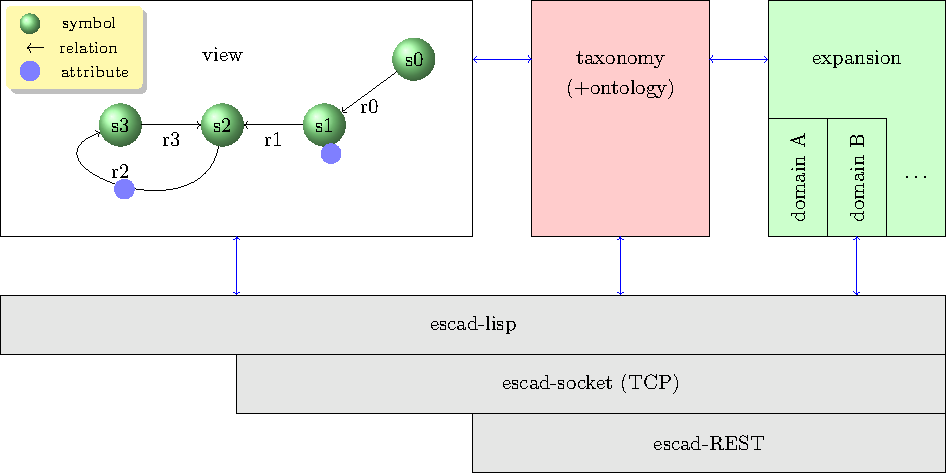
\includegraphics{figures/overview.pdf}
  \caption{Overview of basic escad structure.}
  \label{fig:overview}
\end{figure}
However a short additional security note on the communication blocks: You can communicate with escad through common-lisp. This communication can also piped through a local TCP-connection by the user. Note that for security reasons you should not make such network-communications over the internet, since escad is not encrypted. This is also true for the HTTP connection. It is currently only meant for local network use. However you could use technics like VPN if you want secure transfer through the internet.
\subsection{Symbol - name things to talk about}
The symbol, also called \index{node}node in some papers, can represent a house, a number, a theory, a joke or whatever you want. This allows you to describe the parts of the world for a specific purpose. That shows the great flexibility of escad. In figure~\ref{fig:overview} symbols are circles with names in it (e.g. $s_0$) which you can name however you want, as long it is a unique name in the current graph. In case you do not care, escad can even generate a unique name for you.

Symbols can also be seen as a function (called by \textbf{activation}) which takes an input to produce some output. The input can be given via optional incoming-relations and/or an optional \textbf{activate-slot}\footnote{One can argue that input could solely provided by incoming relation(s). This is true. However escad provides this input method to also enable customizable functionality to single symbols (those which are not connected by relations). Another reason is that many symbols need at least one input, so this design reduces also the complexity of the graph. However if you need one input in different symbols it could be more fails-safe to provide one symbol as input-value and relate to the symbols which need that input.} (meaningful especially if the symbol stands alone wtihout connected relations). The output is written in \textbf{representation} slot and can be transported from there to other symbols via some relations. Optionally side effects are allowed and used to add/delete/modify other symbols or relations.
\subsection{Relation - describe relationships of symbols}
A relation (or in computer science also called \index{edge}edge) creates a relationship or dependency between two symbols. You can specify the taxonomy (meaning) of this dependency further. Try to use the most specific domain expansion for your model in order to get the most advanced tools. However sometimes the detailed model is not clear in detail so that you can use a most generic relation taxonomy.
% Generally one can divide following classes of dependencies:
% \begin{description}
% \item[is\_a] can be used to describe/create symbol-hierarchies (also known as hyperonym–hyponym or supertype/superclass $\rightarrow$ subtype/subclass).
% \item[has\_a] can be used to define a possessive hierarchy/aggregation (no ownership) between symbols (also known as holonym/whole/entity/container $\rightarrow$ meronym/part/constituent/member).
% \item[part\_of] can be used to describe a ownership hierarchy/composition between symbols (also known as meronym/constituent $\rightarrow$ holonym/entity).
% \item[member\_of] can be used to describe a containment (also known as meronym/member $\rightarrow$ holonym/container).
% \item[instance\_of] can be used to describe a concept-object (also known as token/object $\rightarrow$ type/class).
% \end{description}
\subsection{Attribute - for storing your hashtags}
An \index{attribute}attribute in escad is an \emph{optional} specifier of a symbol or relation. It is meant for searching by user-specific tagging of object(s). There can be a huge discusion whether attributes or whether a symbol and relation should be used instead, because attributes are implicite relations. As a rule of thumb, attributes should not be used for controlling the behaviour of a symbol. Take your choice and try to keep this choice consistent over your graph. Consider that attributes may not taken into account by some graph functions. Attributes merely are \emph{keywords} which give the symbol or relation additional information. An indicator to use a relation and a symbol instead of an attribute is, if you want to supply to such a keyword an value. E.g. to describe that a symbol uses/needs a file, you should create a file-symbol and create a use-relation.

The attribute contains text with a special structure. Every attribute-entry (key) begins with a \emph{hasthag} ``\#'' followed by a string with no spaces in it. You can add many such hashtags by seperate them with at least one space char.
\subsection{View - where all lives in}
You can think of the view as a workplace where you can put in symbols and relations, which model an part of the real world. It is called view because it is the current view of a world modelled in your escad session. However like in the real world there are often multiple and different views of the world. Thus you can acess other views through a view-symbol in the standard expansion mentioned later.
\subsection{Taxonomy - semantic of objects}
With taxonomy you assign a semantic (meaning) and classification to your symbols and relations. The available taxonomies you can use depends on the available expansions, because expansions provide also taxonomies. Taxonomy is the basic for the ontology. A taxonomy-designator has following format: \textbf{<domain>:<taxonomy-name>}
\subsection{Ontology - behaviour of objects}
 Depending of the taxonomy there may result different (graphical) output or behaviour (functionality) by escad. This is possible with the ontology provided in the expansions (explained later). In semantic-knowledge field you may hear often words like \index{ontology}ontology. Ontology \emph{uses} the taxonomy to capture and represent the meaning of a domain and has rules what is possible with it and what not. Since escad is aimed to be a practical tool, it has some domain specific ontologie-knowledge included. This knowledge is provided by an expansion.
\subsection{Expansion - customize your needs}
Expansions are a collection of \emph{symbols}, \emph{relations} and \emph{functions} which define a \emph{taxonomy} and a domain specific \emph{ontology}. This assures that one can model with a specific taxonomy and rules of how symbols and relation are combinable and which functionality they provide. This ranges from graphic output to new generated graph-elements. There are many possibilities and you can even write your own expansion(s). Those programms live in the escad environment and can use the provided feature, even of other expansions. However currently there is only a limited set of expansion, but this could increase in time. Feel free to write a expansion for your domain specific needs.

When we speak of \emph{activation} of a expansion, what does that mean? You as user give a activation command or right-klick on the symbol, then a special function is executed. What special function is that and what does it make? Well in fact it is the \emph{activate} function. This function can take additional parameters. You can specify them within the Attribute \emph{activation\_command}. The default value is \emph{neighbourhood} which does what it says: It shows all in- and outgoing relations and the symbols which they are related to.
\subsection{Workspace - all the files}
The workspace is the directory which is used by default for reading or writing of escad. This is convenient for you, but note that existing files can be overwritten, so you should copy them if you want use it in the long-term.
\section{Usage patterns}
To get things done with escad, there are several tasks you have or want to do. In this section we provide you with common interaction concepts in escad. It is very useful that you get familiar with them even if you do not know the exact details. So you know what tasks or problems may arise and which facilities escad provides and suggests for this. Detailed examples you will see in the next chapter.
\subsection{Modeling}
Modeling is probably one of the tasks you will do the most time with escad: You describe in escad your topic/task of interest. This is a very important task. If you model something, look at the given examples in the \path{examples} directory. Use the most approbiate taxonomy. Use expansions to ease your live where possible.
Modelling semantic graphs is not a easy task. Of course you can make easily symbols and relations, but it heavily depends how you use them. In the past many semantic projects are died or got not very sucessfull used at a wide range. Barry Smith stated some reasons (\url{https://www.youtube.com/watch?v=p0buEjR3t8A}) like silo-syndrome, short-half-life-syndrome and reinvent-the-wheel-syndrome. Nowadays there is a sucessfull example in bioinformatic where to show how genes affect our biology (see BFO-ontology). However even with the best ontology you can have problems, if you not use it properly. To use it you should have a clear knowledge on what the terms mean and how to use.
Such problems may also occur with escad. To improve the situation, escad tries to have many examples for several domains and tasks. The aim is to have enough examples so that you have the possibility to adapt it easily to your needs. I believe it makes more sense to use semantics than to have endless discussions what is the ''correct'' taxonomy/ontology.
\subsection{Showing}
Showing partial symbols (or in the opposite meaning 'hiding' all other symbols) can be helpfull to concentrate at your current task and may also good for performance (since escad not need to fetch all actual present symbols). This mechanism is provide by the \emph{\_show} symbol, which you should look for to get more information.
\subsection{Grouping}
The more you model, the more your view will get filled and it is hard to keep an overview what topic of your description they model. You need to handle complexity (and in the end also performance). One method is \emph{grouping} symbols which are in close relation to each other depending on a topic or function. For example if you model a 3D object like a room, you may group all symbols defining a table together. This can be done by the group-symbol.
\subsection{Bookmarking}
As you can imagine, even with grouping you may have the problem to jump to different locations far away from the current one. So manual iterration from symbol to symbol may take time or is frustrating. So escad provides bookmarks, similar to the browser bookmarks. You can store and give them accesible names, under the symbol \emph{\_bookmarks}. To learn more about that, refer to the documentation of this symbol.
\subsection{Selecting}
Some functionalities/expansions which require symbols to operate on, need a possibility to select them. This is possible with the internal \emph{\_selection} symbol. To learn more about that, refer to the documentation of this symbol.
\subsection{Mounting}
Sometimes you want hide complexity by including another view which even may be on another computer/network or in a graph-database/disk/file. To connect this seperate view with your actual view you can mount symbol(s) of it to your current view. This is like a door where you can hide complexity but if you need more you can open and connect your view with it. Mounting is done with a expansion. After usage you can unmount the seperate view. You would want to do this especially when a complex mounted view is connected through a slow network. Then escad will react slowly too, because it has to fetch/write data to it.
\subsection{Saving}
Saves your view (or just parts of it) in native escad common lisp format (.lisp) without lose of data precision.
\subsection{Exporting}
Exports your view (or just parts of it) in a non-escad format. This is usefull for use your view in other programms.
In case you can not do some things in escad yet or other tools may do better, you can export your graph. You can export the view to
\begin{description}
\item[graphviz-dot] is a file format for graphviz, which is powerful in graphically layout and drawing of graphs. Export with a expansion.
\item[SVG] is a vector graphic-format viewable through most modern webbrowsers.
\item[PDF] Export with a expansion.
\end{description}
Consider that while exporting you can loose some information or the information is frozen. This not has to be an bug or limited functionality of escad. This also occurs if the target format not supports some features or mechanisms.
\subsection{Loading}
Loads a view (or just parts of it) in native escad common lisp format (.lisp) without lose of data precision.
\subsection{Importing}
Allows you to get a view stored in a non-escad format.
Because interoperability is important in todays heterogenic software world, there should be a way to get graphs from other software.
Graphviz is powerful in graphically drawing of graphs. You can import those graphs with .dot extension. However only basic functionality of dot is currently supported. Import with a expansion.
\subsection{Reporting}
Means to create/process/analyse new things out of your view. E.g. a report could check your view for data-quality like whether there would occur problems when activate a specific expansion or if there are circular graphs.
\subsection{Generating}
Is used to create new symbols, relations or attributes automatically for you. E.g. if there are many symbols and relations with same taxonomy connected sequentially, you may let generate them by just providing the basic data which differs.
\subsection{Automating}
With \emph{flows} automating in escad is possible without to know how to programm in lisp. Refer to the internal symbol \emph{\_flow} for more information.
\chapter{Getting started}\label{cha:gettingstarted}
Here i assume it is easier to get what escad can do for you, by showing escad in work. Note that the look of the following examples may differ a little from the real software, but the semantic should be the same.
\section{Tutorial ``room planing'' with escad command-line}
We want now do a short session in escad. After installation go to the escad root directory and start escad by typing in a shell in your terminal:
\shellcmdline{./escad}{>}
This starts escad REPL (no special arguments given). After loading of common-lisp and escad, you should switch from the common-lisp in the escad namespace:
\lispcmdline{(in-package :escad)}{ESCAD>}
Now you can execute all escad commands directly. To see some possible existing symbols type following escad-command:
\escadcmdline{(ls)}{(``\_escad'')}\label{ex:ls}\index{command example!ls}
You can read more about this command at page~\pageref{it:ls}. We see a symbol which escad has already created for us. The symbol can contain settings for our current escad session.
However we heard that escad has symbols and relations. Lets look at the relations:
\escadcmdline{(lr)}{NIL}\label{ex:lr}\index{command example!lr}
Upps, we get \emph{NIL} which is the lisp way of saying that there is nothing. But that is ok, since we just have not created anything yet. So lets create three symbols:
\escadcmdline{(dolist (name '(``one'' ``two'' nil)) (cs name))}{NIL}\label{ex:cs}\index{command example!cs}
This produces three new symbols, which names we not see because of the \texttt{dolist} nature:
\escadcmdline{(ls)}{(``\_escad'' ``\_view'' ``one'' ``two'' ``s0'')}\index{command example!ls}
The third symbol name \texttt{s0} created escad for us, because we provided \texttt{nil}.
Now lets create a relation:
\escadcmdline{(cr nil ``one'' ``two'')}{``r0''}\label{ex:cr}\index{command example!cr}
Now we got
\escadcmdline{(lr)}{(``r0'')}
Note that you can not insert a new relation or symbol which name already exists.
You now have nearly seen all basic operations in escad. Most functionality can be achieved by this. Instead of learning many new commands, you can use in escad symbols which can also represent actions (e.g. exporting a PDF of your view). But how can you execute such a symbol. This makes the command \emph{as}, which \emph{activates} the given symbol:
\escadcmdline{(as ``s0'')}{(``Documentation text...'')}
You can activate every symbol, but most of them will just print some documentation about themselves, like you have seen in the last command. To get another functionality you have to assign a taxonomy which refers to a expansion. Those expansion is then loaded and executes a defined command (which is defined by the taxonomy).
You can easily add taxonomy to a symbol with add a \emph{property}:
\escadcmdline{(s ``s0'' :taxonomy ``export.pdf'')}{(``s0'')}
If you would activate this smybol now, it would produce a pdf with graphic output of your current view. Because you gave no file-name it would generate some. To give a filename you can add a special attribute-property:
\escadcmdline{(s ``s0'' :attribute ``my\_file.pdf'')}{(``s0'')}
Now you should get those pdf-file.
This are the most basic commands you need to know in escad. To get detailed command info use command help:
\escadcmdline{(help-command 'cmd\_name)}{(``Documentation text of cmd\_name...'')}
To get basic help type:
\escadcmdline{(help)}{(``Documentation text...'')}

To enter the data for our room-tutorial you should refer to listing~\ref{listing:tutorial} shows a minimal expansion.
%and the listing~\ref{listing:exp_tax} shows the entry in a taxonomy file.
\begin{lstlisting}[caption={Code for the room-tutorial.}, language=Lisp, morekeywords={do-external-symbols, find-package, in-package, slot-value, use, with-slots}, label=listing:tutorial]
(activate-value (s "_expansion") "room_expansion.lisp")
(as (s "_expansion"))  ; load room-expansion
(cs "c0" :activate "0, 0" :taxonomy "room:corner" :comment "lower-left point of the room (base)")
(cs "c1" :activate "0, 8" :taxonomy "room:corner")
(cs "c2" :activate "8, 8" :taxonomy "room:corner")
(cs "c3" :activate "8, 5" :taxonomy "room:corner")
(cs "c4" :activate "6, 5" :taxonomy "room:corner")
(cs "c5" :activate "6, 0" :taxonomy "room:corner")
(cs "d0" :activate "1, 0" :taxonomy "room:door" :label "D")
(cr "
\end{lstlisting}
%To load stored views or escad-lisp-scripts (e.g. in the \emph{examples} directory) type:
%\escadcmdline{(lov ``mindmap.lisp'')}{(...)}
%To list available taxonomies use command \texttt{(lta)}.
\section{Tutorial ``room planing'' with graphical browser-interface}
We want now do a web-session in escad. If you already followed the previous command-line section, escad is running and you can skip the following step. So if escad is not running yet go to the escad root directory and start escad by typing in a shell in your terminal:
\shellcmdline{./escad}{>}
This starts escad and a http-server if you have the default settings in your \path{escad\_conf.lisp} (with the symbol \emph{\_web} activated).

Now in your web-browser you can enter \texttt{127.0.0.1:4242/} to request the html-page which at first time loads a web-client in your browser. After loading is finished you can view and edit the graph like in figure~\ref{fig:escad_gui}. If you already executed the command-line tutorial you now already see the graph. If you have entered no such room-data, in principal we can create now the data in this graphical user interface by hand. To ease our live we enter the data in the command-line by copy and paste the listing~\ref{listing:tutorial} from the previous command-line tutorial. Now you can play around with it and maybe edit the corners of the room by clicking on the symbol and enter new values.
\section{FAQ}
Sometimes questions lead to a fast recognition of a problem or help to understand things better. Not all questions may be frequently asked, but who cares :-)
\subsection{Scope}
\begin{description}
\item[Does it not make more sense to store the graph in a graph database?] In some cases it could make sense. However escad is not meant to be a high performance graph storage tool. Think escad as a workshop where there are many tools and workpieces. A graph database is just one specific high efficient tool. Escad is the host from which the user can interact in a unique interface with many of such tools. In fact it is planned to implement a mounting facility for graph databases. So that you can additionaly store your view in it.
\item[I really do not understand whether escad is for me?] Do you search a nice software to make crazy pictures of your graph in a interactive way? Then you currently may not be right here, just look at something like gephi. Escad is for people who want to work exactly and reproducible with graphs in a more describing manner and in a second step there will be an output (similar like batch processing).
\item[Can i make complex queries like in a graph database?] Perhaps you need a graph database, escad is not a pure graph database. It is a tool, not designed as a speed optimized storage container. However it is planed to have a graph-database connection (e.g. to great arangodb) in order to support persistent huge graphs.
\end{description}
\subsection{Usage}
\begin{description}
\item[Is there a difference in the power of the different escad interfaces?] Yes! But as you can imagine by the fact that there \textbf{are two different interface flavours} like the \textbf{command line} and \textbf{web gui} interface each one has it advantage and usage. Each interface has it strength, thus it makes sense to use all. Where the commandline has powerful scripting capabilities, the web-interface allows a more intuitive and haptical way to interact with the graph and explore it easily.
\item[Why you have choosen common-lisp as the language for escad?] While having some experience with different languages, lisp has one of the simplest syntax for me. The REPL allows interactive rapid prototyping. Lisp is an old, standardzied, stable and mature language. One can simply extend it for future needs and implement easily a domain specific language (DSL) if needed.
\end{description}
\subsection{Development}
\begin{description}
\item[Can i help develop escad?] Of course, very welcome! This currently is a project done in spare free time beneath work. So just contact the developer in github to improve escad together.
\end{description}
\subsection{Other}
\begin{description}
\item[Is there support for other languages as english?]  No not currently. The main author is german, but has spare time to keep manual in german as well. Currently english is choosen to reach a wide international range of people. If you want contribute with translation for your language feel welcome.
\end{description}
\chapter{Reference}
Note in order to understand the reference you should be familiar with the section~\ref{sec:concept}. Here you find the detailed information to work with escad, such as available commands or interfaces. Also you should get some basic things in order to get the idea in how you can extend escad or help in development.
See figure~\ref{fig:overview} for how escad is structured. Basically you get with escad two parts of software. The lisp side as \emph{server} and in case of the gui the javascript side, which acts as a \emph{client}.
\section{View in detail}
The figure~\ref{fig:graphdetail} shows the default view in detail. It lives in the server and holds all your symbols and relations. You can see the default automatically generated symbols which are explained later. For the first left relation there are the reference slot names given (printed in red). The symbol \emph{\_escad} has no incoming references, thus there is just the \emph{ref\_to} slot with relations. Further you see the first relation which has both references bound to a symbol and this is usual for relations. This relations references to the symbol \emph{\_view} which thus has just \emph{ref\_from} slot filled.
\begin{figure}[htbp]
  \centering
  \includegraphics[scale=0.8]{figures/graphdetails.pdf}
  \caption{Default view and reference-slot names (red colored).}
  \label{fig:graphdetail}
\end{figure}
Note that the view is your main workplace. There may exist other escad views in other computers. In future escad-versions you may even mount this other views (from file or internet) or from other software tools. In order to acess all the symbols and relations, escad requires a \emph{unique ID}. Even if symbols or relations could technically have the same id, it is adviced to not do this. Some graph-databases do not allow same id for symbols or relations. In that case data exchange with that tools would not work or cause additional work to solve this.
\section{Symbol in detail}
Table~\ref{tab:symbol} shows the symbol slots (properties) meant for editing by the user and their meaning.
\begin{table}[htbp]
\definecolor{light-gray}{gray}{0.9}
\rowcolors{2}{light-gray}{black!20} % alterniert Farbe der Tabellenzeilen
\centering
\begin{tabular}{|p{4cm}|p{12cm}|}
  \hline
  \textbf{slot (property)} & \textbf{description} \\
  \hline
  activate & When a symbol is activated this slot-content is submitted to the activation function. \\
  \hline
  attribute & Used sometimes by expansions for their work. It can hold different objects, just text or even complex objects. \\
  \hline
  comment & Tells something additional about the symbol. This is only meant for the user and should not changed by some automatic code. \\
  \hline
  label & Alternative name which has not to be unique. This can be used by the user to provide longer names or multiple identical names (for whatever reason) but however it is possible to use same name like symbol-id too. \\
  \hline
  representation & Text representing the symbol. The main data slot which contains data by the semantic which is classified by the taxonomy. \\
  \hline
  taxonomy & Classifies the symbol and determines which activation-function will be called. If there is no taxonomy given, then symbol-activation does nothing. \\
  \hline
  visual\_cli & Data how a symbol is visualized in the command line interface. \\
  \hline
  visual\_web & A JSON string specifying data how a symbol is visualized in the web interface (position,....). \\
  \hline
  weight & A number which denotes, depending on the usage, the importance / weight / order of the symbol. \\
  \hline
\end{tabular}
\caption{Slots of the symbol object.}
\label{tab:symbol}
\end{table}
\section{Relation in detail}
In escad every relation is technically \emph{directed}. But this is just to store the direction in case you need it. Of course you can also model undirected or bidirectional graphs in escad. To do this you can use expansions which ignore the direction of the relation or you can use a special undirected- or bidirectional taxonomy or you can create two relations with the opposite direction to model bidirectionally. Escad also supports \emph{multigraphs}, so that there are multiple relations to/from the same target/source.

Table~\ref{tab:relation} shows the relation slots (properties) meant for editing by the user and their meaning.
\begin{table}[htbp]
\definecolor{light-gray}{gray}{0.9}
\rowcolors{2}{light-gray}{black!20} % alterniert Farbe der Tabellenzeilen
\centering
\begin{tabular}{|p{4cm}|p{12cm}|}
  \hline
  \textbf{slot (property)} & \textbf{description} \\
  \hline
  attribute & Used sometimes by expansions for their work. \\
  \hline
  comment & Tells something additional about the symbol. \\
  \hline
  label & Alternative name which has not to be unique. \\
  \hline
  representation & Text representing the symbol. \\
  \hline
  taxonomy & Classifies the symbol and shows to which expansion it belongs. \\
  \hline
  visual\_cli & Data how a relation is visualized in the command line interface. \\
  \hline
  visual\_web & A JSON string specifying data how a relation is visualized in the web interface (position,....). \\
  \hline
  weight & A number which denotes depending on the usage the importance / weight / order of the symbol. \\
  \hline
\end{tabular}
\caption{Slots of the relation object.}
\label{tab:relation}
\end{table}
\section{Internal symbols (``\_''<name>)}
Escad pushes it's concept of \emph{all can be described as graph} clearly forward. So even escad itself shows errors or other informations about itself with \emph{auto generated symbols} beginning with the character \emph{\_}. Thus you can for example check if an command created an error by search for the symbol \emph{\_error}. In the slot \emph{representation} you can see the detailed error message. You have not to delete it after the error occurs but you can (in case to know that a new error exists another time). If a new error occurs the symbol will be populated with new message. All this symbols can be populated from escad in the graph and are connected by a relation to the parent symbol \emph{\_escad}.
Table~\ref{tab:internal-symbols} shows all internal symbols in the current version of escad.
\begin{table}[htbp]
\definecolor{light-gray}{gray}{0.9}
\rowcolors{2}{light-gray}{black!20} % alterniert Farbe der Tabellenzeilen
\centering
\begin{tabular}{|p{4cm}|p{12cm}|}
  \hline
  \textbf{symbol} & \textbf{description} \\
  \hline
  \_error & An error occured. If the error is generated from a expansion, a relation will be added from this symbol to the corresponding expansion symbol. \\
  \hline
  \_escad & Root symbol from which all other internal escad symbols are connected. \\
  \hline
  \_expansion & This is the root symbol from which you cann explore all actual loaded expansions and their functions. Relations are drawn to their taxonomies (which are rootet under the \_taxonomy symbol). \\
  \hline
  \_flow & Connect symbols with this symbol to generate automatic symbol-activation of connected symbols, just like a (work-) flow. \\
  \hline
  \_help & Root symbol for help about escad. \\
  \hline
  \_message & Holds actual generated info messages about escad. \\
  \hline
  \_mount & Childrens of this symbol show all mounted views (if any). \\
  \hline
  \_selection & You can preselect symbols or relations for further actions. The selection for symbols and relations is different. by creating a symbol with taxonomy \emph{std.symbol} or \emph{std.relation} with the object name you want select in slot \emph{representation}. After that create relation to the symbol \emph{\_selection}. \\
  \hline
  \_show & Escad allows everytime acess to all symbols in current view. However this can be a nightmare when many symbols are there. So escad provides mechanisms to manage this complexity. Showing allows to selectively display symbols while the symbols are still acessable by the algorithms. The symbols you want to be shown you have to connect with a relation to this symbol. You not have to connect the internal symbols, because they will be shown at avery time. Note that there is the representation-slot which controls the depth of child-symbols you can see (default is \emph{all} which shows all symbols whereby \emph{1} shows just the first child-symbols). \\
  \hline
  \_taxonomy & This is the root symbol from which you cann explore all actual loaded taxonomies provided by the loaded expansions to which a relation is pointing. \\
  \hline
  \_view & Root symbol of view related things. You can find all \emph{mounted} views there als child nodes. \\
  \hline
  \_warning & Warning message. \\
  \hline
  \_web & Controls the server for the graphical web-interface. Activated with \emph{activate-slot} \texttt{start} starts server, \emph{activate-slot} set to \texttt{stop} ends the server. The \emph{attribute-slot} can hold the root directory for the web-server (where your index.html lives). \\
  \hline
\end{tabular}
\caption{Auto generated internal symbols of escad.}
\label{tab:internal-symbols}
\end{table}
\section{Expansion}
Expansions are a domain specific extension to escad. Basically a expansion contains taxonomy for symbols and relations. This is merely a classification which determines how escad works with those objects. If a symbol has no taxonomy then it is considered as the most general symbol. A taxonomy narrows the semantic of a symbol. The more detailed taxonomy, the more functionality you may get with an expansion.

There are expansions which are included/shipped with escad. Table~\ref{tab:expansion_overview} shows the available expansions included in the current version of escad.
\begin{table}[htbp]
\definecolor{light-gray}{gray}{0.9}
\rowcolors{2}{light-gray}{black!20} % alterniert Farbe der Tabellenzeilen
\centering
\begin{tabular}{|p{2.5cm}|p{6cm}|p{7cm}|}
  \hline
  \textbf{domain} & \textbf{file} & \textbf{description} \\
  \hline
  doc2d & \path{document-2d_expansion.lisp} & Provides common functionality for 2d documents (text structure, tables, graphics). \\
  \hline
  export & \path{export_expansion.lisp} & Export graph to PDF and SVG. \\
  \hline
  import & \path{import_expansion.lisp} & Import graphviz dot-file in view. \\
  \hline
  room & \path{room_expansion.lisp} & Provides functionality for working with rooms (define rooms, doors, windows, furnitures). \\
  \hline
  std & \path{standard_expansion.lisp} & Provides common functionality for broad usage even for other expansions, thus called \textbf{st}andar\textbf{d} expansion. \\
%  3D & \path{3d_expansion.lisp} & Generate 3D files. & 0.2 \\
%  \hline
%  flow & \path{flow_expansion.lisp} & Automates processes in escad. & 0.1 \\
%  \hline
%  generation & \path{generator_expansion.lisp} & Generate objects in view. & 0.1 \\
%  \hline
%  \hline
%  import & \path{mount_expansion.lisp} & Mount other graphs into view like from a graph database. & 0.1 \\
%  \hline
%  report & \path{report_expansion.lisp} & Report view to latex and PDF. & 0.1 \\
%  \hline
%  standard & \path{standard_expansion.lisp} & Provides common useful concepts like sets, checks or canonizing. & 0.1 \\
  \hline
\end{tabular}
\caption{Contained expansions in escad and their functionality sorted by the domain.}
\label{tab:expansion_overview}
\end{table}
Of course there can exist many more not shipped one. This external expansions you have to copy into expansion dir and to load with the load expansion. After that you can check which additional expansions are loaded in escad yourself by exploring the \emph{\_escad} symbol (how this is done you can see in the \ref{cha:gettingstarted}). Escad not atomatically reloads changed files, to do this just activate once more the load expansion to get the most up to date state.
To include external expansions, it is the same process like including the included internal expansions.

In the following subsections this included expansion are explained in detail, whereby following table headings are used:
\begin{description}
\item[obj] (short for \textbf{object}) is either a symbol also denoted as \textbf{s}, a relation which is denoted as \textbf{r} or a function which is denoted as \textbf{f}.
\item[taxonomy] is the unique taxonomy-designator of the object (consisting of <domain>:<name>).
\item[in] shows which objects are allowed, according the ontology, to connect in the object. If there is nothing given, it is not specified and you can do whatever you want. Multiple in- or outgoing objects are seperated by comma.
\item[out] shows which relations are allowed to point out of the expansion to other symbols/expansions. If there is none, the symbol is meant to stay unique.
\item[act] (short for \textbf{activate}) is a string \textbf{F} which denotes a file-name or a string \textbf{S} with explained meaning in the desccription-column. In case of an optional string it is placed inside brackets ([ ]). A empty field means a given string is ignored by activation.
\item[description] explains what the specific object does.
\end{description}
\subsection{std expansion}
In the following table~\ref{tab:standard-expansion} the included std-expansion is shown. It contains symbols and relations which are helpful in many domains and helps the user to be faster in generating graphs. Following Abbreviations are used:
\begin{description}
\item[$A_0$] = "", this means no input at activate-slot (empty string).
\item[$A_1$] = "start".
\item[$A_2$] = "stop".
\item[$I_0$] means all taxonomies as input.
\end{description}
\begin{table}[htbp]
\definecolor{light-gray}{gray}{0.9}
\rowcolors{2}{light-gray}{black!20} % alterniert Farbe der Tabellenzeilen
\centering
\begin{tabular}{|p{1cm}|p{3cm}|p{1.5cm}|p{1.5cm}|p{1cm}|p{7cm}|}
  \hline
  %\rotatebox{90}{\textbf{object\ }} & \textbf{taxonomy designator} & \textbf{in} & \textbf{out} & \rotatebox{90}{\textbf{representation\ }} & \textbf{description} \\
  \textbf{obj} & \textbf{taxonomy} & \textbf{in} & \textbf{out} & \textbf{act} & \textbf{description with \texttt{slots}} \\
  \hline
  \textbf{s} & std:load & & & $A_0$ & $A_0$: Load a lisp \texttt{file} (e.g. expansion). \\
  \hline
  \textbf{s} & std:text & & & $A_0$ & UTF-8 encoded text in \texttt{representation}, text is always representing itself. \\
  \hline
  \textbf{s} & std:webserver & & & $A_0$ - $A_2$ & $A_0$-$A_2$: \texttt{representation} get status (running or stopped).\newline $A_1$: \textbf{start} server.\newline $A_2$: \textbf{stop}'s the internal webserver for the graphical user interface. \\
  \hline
\end{tabular}
\caption{Standard expansion.}
\label{tab:standard-expansion}
\end{table}
\subsection{import expansion}
The table~\ref{tab:import-expansion} shows the included graph-import facilities for escad.
% \newcommand{\tabitem}{~~\llap{\textbullet}~~}
% \begin{table}[htbp]
% \centering
% \begin{tabular}{rp{11cm}}
%   \toprule
%   \textbf{taxonomy} & \colorbox{black!20}{escad.symbol.\_escad.export.dot} \\
%   \textbf{in} & - \\
%   \textbf{out} & - \\
%   \textbf{attribute} & 1. symbol name \\
%                      & 2. [file name] \\
%   \textbf{description} & exports view to dot (graphviz) \\
%   \midrule
%   \textbf{taxonomy} & \colorbox{black!20}{escad.symbol.\_escad.export.pdf} \\
%   \textbf{in} & - \\
%   \textbf{out} & - \\
%   \textbf{attribute} & 1. symbol name \\
%                      & 2. [file name] \\
%   \textbf{description} & exports view to pdf \\
%   \midrule
%   \textbf{taxonomy} & \colorbox{black!20}{escad.symbol.\_escad.export.svg} \\
%   \textbf{in} & - \\
%   \textbf{out} & - \\
%   \textbf{attribute} & 1. symbol name \\
%                      & 2. [file name] \\
%   \textbf{description} & exports view to svg. \\
%   \bottomrule
% \end{tabular}
% \caption{Symbols and relations of export expansion.}
% \label{tab:exp-export-expansion}
% \end{table}
%\subsection{flow\_expansion.lisp}
%Todo...
%\subsection{generator\_expansion.lisp}
%Todo...
\begin{table}[htbp]
\definecolor{light-gray}{gray}{0.9}
\rowcolors{2}{light-gray}{black!20} % alterniert Farbe der Tabellenzeilen
\centering
\begin{tabular}{|p{1cm}|p{3cm}|p{1.5cm}|p{1.5cm}|p{1cm}|p{7cm}|}
  \hline
  \textbf{obj} & \textbf{taxonomy} & \textbf{in} & \textbf{out} & \textbf{act} & \textbf{description} \\
  \hline
  \textbf{s} & import:dot &  &  & \textbf{F} & import from dot (graphviz). \\
  \hline
\end{tabular}
\caption{Import expansion.}
\label{tab:import-expansion}
\end{table}
%\subsection{report\_expansion.lisp}
%Todo...
\subsection{export expansion}
Table~\ref{tab:export-expansion} shows the included export-expansion for exporting the view into different document-formats.
\begin{table}[htbp]
\definecolor{light-gray}{gray}{0.9}
\rowcolors{2}{light-gray}{black!20} % alterniert Farbe der Tabellenzeilen
\centering
\begin{tabular}{|p{1cm}|p{3cm}|p{1.5cm}|p{1.5cm}|p{1cm}|p{7cm}|}
  \hline
  \textbf{obj} & \textbf{taxonomy} & \textbf{in} & \textbf{out} & \textbf{act} & \textbf{description} \\
  \hline
  \textbf{s} & export:dot & & & \textbf{F} & exports view to dot (graphviz). \\
  \hline
  \textbf{s} & export:pdf & & & \textbf{F} & exports view to pdf. \\
  \hline
  \textbf{s} & export:svg & & & \textbf{F} & exports view to svg. \\
  \hline
\end{tabular}
\caption{Export expansion.}
\label{tab:export-expansion}
\end{table}
\subsection{document-2d expansion}
Table~\ref{tab:document-2d-expansion} shows the included expansion for describing two dimensional features like text, pictures or tables.
\begin{table}[htbp]
\definecolor{light-gray}{gray}{0.9}
\rowcolors{2}{light-gray}{black!20} % alterniert Farbe der Tabellenzeilen
\centering
\begin{tabular}{|p{1cm}|p{3cm}|p{1.5cm}|p{1.5cm}|p{1cm}|p{7cm}|}
  \hline
  \textbf{obj} & \textbf{taxonomy} & \textbf{in} & \textbf{out} & \textbf{act} & \textbf{description} \\
  \hline
  \textbf{s} & doc2d:text & & & \textbf{F} & Simple text. \\
  \hline
  \textbf{s} & doc2d:figure & & & \textbf{F} & Figure to insert in a document in PDF format. \\
  \hline
  \textbf{s} & doc2d:table & & & \textbf{F} & Describes a table. \\
  \hline
\end{tabular}
\caption{Two dimensional documents expansion.}
\label{tab:document-2d-expansion}
\end{table}
\subsection{room expansion}
In the following table~\ref{tab:room-expansion} the included room-expansion is shown. It contains symbols and relations which are helpful in to describe rooms.
\begin{table}[htbp]
\definecolor{light-gray}{gray}{0.9}
\rowcolors{2}{light-gray}{black!20} % alterniert Farbe der Tabellenzeilen
\centering
\begin{tabular}{|p{1cm}|p{3cm}|p{1.5cm}|p{1.5cm}|p{1cm}|p{7cm}|}
  \hline
  \textbf{obj} & \textbf{taxonomy} & \textbf{in} & \textbf{out} & \textbf{act} & \textbf{description} \\
  \hline
  \textbf{s} & room:corner & & & & Describes a corner of the room. \\
  \hline
  \textbf{s} & room:door & & & & Describes a door of the room. \\
  \hline
  \textbf{s} & room:object & room:\-wall-to & room:\-wall-to & & Defines a furniture, machine or something in the room. \\
  \hline
  \textbf{s} & room:window & & & & Describes a window of the room. \\
  \hline
  \textbf{r} & room:wall-to & & & & Describes a wall from one point to another. You have to define a closed room by connect corner's with this relation without breaks (other than doors or windows) counterclockwise. \\
  \hline
\end{tabular}
\caption{Room expansion.}
\label{tab:room-expansion}
\end{table}
\section{HTML-webclient usage}
Take your browser to communicate with escad in a graphical intuitive way. This starts only a http-server if you have the default settings in your \path{escad_conf.lisp} (with the symbol \emph{\_web} activated). With your web-browser you can browse the page at \texttt{127.0.0.1:4242/} which at first time loads a web-client in your browser. After that you can view and edit the graph like in figure~\ref{fig:escad_gui}.
\section{LISP command-line and server usage}\label{sec:cmd_line}
The command-line provides the full functionality. This means you got a common-lisp REPL with escad-package loaded. This gives you the full power of common-lisp with the ability of the escad-commands to work with a simple graph environment.
\subsection{Starting and lifecycle of escad}
In a unix manpage manner, escad could be shortly described like in \ref{fig:manpage}.
\begin{figure}[htbp]
  \begin{shaded*}
    % \parbox{14cm}{\underline{\Large{TEST}}}
    \texttt{ESCAD(1)}\hspace{110mm}\texttt{ESCAD(1)}\newline
    
    \textbf{\texttt{NAME}}\newline
    \hspace*{5mm}
    \begin{minipage}{14cm}
      \textbf{\texttt{escad}} - the command-line interface with integrated server for web-interface.
    \end{minipage}\newline\newline
    
    \textbf{\texttt{SYNOPSIS}}\newline
    \hspace*{5mm}
    \begin{minipage}{14cm}
      \textbf{\texttt{escad}} [\underline{escad-lisp-commands}]
    \end{minipage}\newline\newline
      
    \textbf{\texttt{DESCRIPTION}}\newline
    \hspace*{5mm}
    \begin{minipage}{14cm}
      Escad is the \textbf{e}xpansible \textbf{s}ymbolic \textbf{c}omputer \textbf{a}ided \textbf{d}escription tool. It provides you a common-lisp repl after starting. For initial commands you can use the argument \underline{escad-lisp-commands} which is executed in the escad-namespace. A integrated web-server is provided too, so that you can work with your escad view also in a graphical user interface. Choose the one which fits best for your workflow. Note that you can also use stdin to execute escad scripts.
    \end{minipage}
      % \vspace{0.5cm}
    \end{shaded*}
  \caption{escad unix manpage.}
  \label{fig:manpage}
\end{figure}
In following the lifecycle of an escad session is explained.
\begin{enumerate}
\item Escad is started.
\item Init internal symbols.
\item If an single optional argument-string is given evaluate it (e. g. for setting internal symbols like \_view).
\item Load view (default \path{view.lisp}) from workspace.
\item Read config file \path{escad_conf.lisp} (e. g. for starting web gui).
\item Print welcome and enter waiting for input in common-lisp REPL.
\item Escad is ended (interactive, script or expansion).
\end{enumerate}
\subsection{ESCAD common-lisp subcommands}
The table~\ref{tab:cmd_abbreviatons} explains used symbols, abbreviations and the data-structures in the reference.
\begin{table}[htbp]
%\definecolor{light-gray}{gray}{0.9}
%\rowcolors{2}{light-gray}{black!20} % alternates color
\centering
\begin{tabular}{lp{6cm}p{6cm}}
  \textbf{PATTERN} & \textbf{DESCRIPTION} & \textbf{EXAMPLE} \\
  \toprule
  %ATTR & attribute taxonomy string & \texttt{``escad.attribute.author''} \\
  %\midrule
  \textbf{cmd} & command name & \textbf{asa} \\
  \midrule
  %(ATTR STRING ...) & attribute taxonomy value list & \texttt{(``escad.attribute.author'' ``Author Name'')} \\
  %\midrule
  NIL & common lisp nil means not true/done & \texttt{NIL} \\
  \midrule
  RN & relation name string & \texttt{``r0''} \\
  \midrule
  SN & symbol name string & \texttt{``s0''} \\
  \midrule
  RO & relation object & \texttt{``r0''} \\
  \midrule
  SO & symbol object & \texttt{``s0''} \\
  \midrule
  STRING & string with unspecified or multiple semantic & \texttt{``a message string...''} \\
  \midrule
  %VN & view number & \texttt{0} \\
  %\midrule
  + & previous content can occur at least once or multiple times & \\
  \midrule
  * & previous content can occur not or multiple times & \\
  \midrule
  ... & previous pattern can be continued & \texttt{(0 1 2 ...)} \\
  \midrule
  () & basic common-lisp list & \texttt{(1 ``Hello'')} \\
  \midrule
  \lbrack\ \rbrack & optional argument(s) & \texttt{(cmd \lbrack\ \rbrack)} \\
  \midrule
  \colorbox{black!20}{function argument} & function argument & \\
  \midrule
  \colorbox{green!20}{function result} & function result, multiple values seperated by comma are possible & \\
  \bottomrule
\end{tabular}
\caption{Explained abbreviations and symbols.}
\label{tab:cmd_abbreviatons}
\end{table}
In general escad provides two flavours of commands: object- or text-based. There is no superior flavour, just use the one which fits your concrete needs the best. This command reference is sorted alphabetically, so the order of commands does not say something about the quality or importance of them.
\begin{description}% \item[$\to$]
%\item[\parbox{8.5mm}{ad}] \label{it:ad} \escadcmd{ad}{}{STRING}{<a>nalyze <d>iameter (length of longest path(s)) of current view and returns multiple values: the diameter of longest path(s) and the path(s) itself.}
\item[\parbox{8.5mm}{as}] \label{it:as} \escadcmd{as}{\lbrack\ SN \rbrack}{STRING}{<a>ctivate <s>ymbol in current view.
What happens depends on the taxonomy of the symbol. Many symbols print out a string as their contents.
Symbols which represent expansions will execute the configured function of the expansion.}
%\item[\parbox{8.5mm}{asa}] \label{it:asa} \escadcmd{asa}{SN (ATTR STRING ...)+}{SN | NIL}{<A>dd/edit <s>ymbol <a>ttributes depending of key. NIL if nothing is added.}
%\item[\parbox{8.5mm}{gra}] \label{it:gra} \escadcmd{gra}{RN attribute-string}{STRING}{<G>et <r>elation <a>ttributes depending of given attribute-string.}
%\item[\parbox{8.5mm}{gsa}] \label{it:gsa} \escadcmd{gsa}{SN attribute-string}{STRING}{<G>et <s>ymbol <a>ttributes depending of given attribute-string.}
\item[\parbox{8.5mm}{cr}] \label{it:cr} \escadcmd{cr}{RN | nil SN SN \lbrack\ :attribute :comment :taxonomy :weight \rbrack}{RN | nil}{<C>reate <r>elation with given name and possible additional values in view. If the relation-name already exists do nothing and return nil. Default type is undirected relation. To make a directed or bidirected relation, set the appropriate taxonomy (note that ref\_from and ref\_to are only technical terms meaning you first tie the relation from that symbol to another. it can mean that is directe, but it is not guaranted that the author means that unless he makes that explicit with a relation that declares that).}
\item[\parbox{8.5mm}{cs}] \label{it:cs} \escadcmd{cs}{SN | nil \lbrack\ :attribute :comment :taxonomy :weight \rbrack}{SN | nil}{<C>reate <s>ymbol with given name and possible additional values in view. If the symbol-name already exists do nothing and return nil.}
%\item[\parbox{8.5mm}{help}] \label{it:help} \escadcmd{help}{}{STRING}{Print <help>ful overview of escad, meaning of terms and all available commands.}
%\item[\parbox{8.5mm}{lov}] \label{it:lov} \escadcmd{lov}{STRING}{STRING | nil}{<LO>ad <v>iew from the file given as string.}
\item[\parbox{8.5mm}{lr}] \label{it:lr} \escadcmd{lr}{\lbrack\ :filter :exclude-taxonomy \rbrack}{(RN*)}{<L>ist all <r>elations in current schematic which name match the filter. Additionally exclude relations which match the exclude-taxonomy.}
\item[\parbox{8.5mm}{ls}] \label{it:ls} \escadcmd{ls}{\lbrack\ :filter :exclude-taxonomy \rbrack}{(SN*)}{<L>ist all <s>ymbols in current schematic which name match the filter. Additionally exclude symbols which match the exclude-taxonomy.} See example at page~\pageref{ex:ls} for usage.
\item[\parbox{8.5mm}{r}] \label{it:r} \escadcmd{r}{RN \lbrack\ :comment :ref\_from :ref\_to :taxonomy :weight \rbrack}{RO | nil}{Get/set <r>elation object.}
\item[\parbox{8.5mm}{s}] \label{it:s} \escadcmd{s}{SN \lbrack\ :comment :taxonomy :weight \rbrack}{SO | nil}{Get/set <s>ymbol object.}
\item[\parbox{8.5mm}{rr}] \label{it:rr} \escadcmd{rr}{RN}{RN | nil}{<R>emove <r>elation.}
\item[\parbox{8.5mm}{rs}] \label{it:rs} \escadcmd{rs}{SN}{SN | nil}{<R>emove <s>ymbol.}
%\item[\parbox{8.5mm}{sav}] \label{it:sav} \escadcmd{sav}{STRING}{STRING | nil}{<SA>ve <v>iew to the file given as string.}
\end{description}
\section{Library usage}
To use escad as a library in your common lisp programm, just load \path{package.lisp}.
\chapter{Development}
Everyone is needed and welcome for escad development. If you are a graphical designer, you are got in documenting or you like to program in lisp or you are interested in web-programming - all is required in escad. :-)
The project is managed with the famous source-code management tool \emph{git} (also known as used in the linux kernel development). The repository is hosted under \url{https://github.com/mkollmar/escad}.

A \emph{Makefile} contains the basic task to generate the code or documentation. So it may be a good choice to look into it in order to get a basic idea how all works. Nevertheless the next sections contain how the development process is (currently) structured. It follows a brief overview over the directory structure and a explanation what it contains (or should contain in the future). The last section provides information in how to program a expansion and the interface
\section{Development process and quality}
As mentioned at page~\pageref{sec:ddd} escads development follows the documentation-driven approach.
All follows this process in short:
\begin{enumerate}
\item Set/increment version according to semantic versioning \parencite{web:semver}
\item Update/create documentation (this manual)
\item Develop code and test along documentation and go back to the previous step when needed.
\item Test and go back one or two steps when needed.
\item Tag version and deliver it.
\end{enumerate}
A note to tests, as it seems to become one big factor of good code quality. Surely test are a good method to check well defined interfaces. So here we implement tests too. However because at the early development stage of escad and limited man power, tests will not take as much room as there could be. Since interfaces may change often we will concentrate at often used functions and in more stable versions of escad the tests should be increased.
\section{Files and directories}
The directory structure and some basic files of the repository will be explained in this section. In the root of the repository there are following files with their purpose:
\begin{description}
\item[Makefile] contains the instructions for the \emph{make} programm and controls the most part of escad development process (generating documentation, binary or other things). Just enter \texttt{make} in the command line to see available options.
\item[LICENSE] holds the license to which terms you have to use escad.
\item[README.md] is mostly for github where escad is hosted and contains shor overview about the project.
\item[doc/] contains the escad documentation for user and developer. Currently this is mainly this manual written in \emph{latex}. But in future a unix man-page, more examples or online documentation would be great, too.
\item[lisp/] contains the escad-lisp files with the implementation.
\item[lisp/escad\_conf.lisp] can contain user settings which are executed at startup.
\item[lisp/expansion/] contains all escad-expansions which are available.
\item[lisp/examples/] contains examples which can be loaded in escad. But note that currently not all may work yet, they are more a print what a future interface should look like.
\item[misc/] contains miscellaneous things which have no other place where it fits.
\item[test/] has unit tests, which execution may be controlled with make.
\item[web/] with the web based graphical user interface (gui) things, which are executed in the web-browser, live here. \path{index.html} is the starting point for the gui and will be served first bei the server.
\end{description}
\section{Programming your own expansion}
Writing escad expansions means simply regular common-lisp CLOS-usage. That means defining classes and methods. Go through following steps carefully and you will have a good basis for writing your own. The code in listing~\ref{listing:exp_minimal} shows a minimal expansion.
%and the listing~\ref{listing:exp_tax} shows the entry in a taxonomy file.
\begin{lstlisting}[caption={Minimal expansion code of a taxonomy called ``test''.}, language=Lisp, morekeywords={do-external-symbols, find-package, in-package, slot-value, use, with-slots}, label=listing:exp_minimal]
(in-package "COMMON-LISP-USER")
(defpackage :de.markus-herbert-kollmar.escad.test
(:use :common-lisp :escad)
  (:nicknames :test)
  (:export :test-class :test-function)
  (:documentation "This is my test expansion."))
  
(in-package :de.markus-herbert-kollmar.escad.expansion.test)

(defclass my-function (symbol-name-string)
"This function will be executed by calling this expansion.")

(defgeneric activate (test-class)
  (:documentation "Test class activation function."))
  
(defmethod activate ((obj test-class))
  (with-slots ((rep representation) (act activate)) obj
    (setf (representation obj) "Test")))

;;;; Symbol management functions ;;;;
(defun list-taxonomies ()
  "Return list of all external taxonomies in this package."
  (let (classes) 
    (do-external-symbols (s (find-package "TEST"))
      (when (find-class s nil)
        (push s classes)))
    classes))

(defun list-functions ()
  "Return list of all external functions in this package."
  (let (functions) 
    (do-external-symbols (s (find-package "TEST"))
      (when (fboundp s)
        (push s functions)))
    functions))

;;;; Set _message symbol to the loaded expansion ;;;;
(setf (slot-value (escad:s "_message") 'representation) 'std)
\end{lstlisting}
% \begin{lstlisting}[caption={Entry in a taxonomy-file.}, language=Lisp, morekeywords={}, label=listing:exp_tax]
% (:taxonomy "escad.symbol.hello_world" :doc "[E] Hello world."
% :expansion "hello_world_expansion.lisp"
% :package :de.markus-herbert-kollmar.escad.hello_world
% :function "my_function"
% :license "GNU GPL 3")
% \end{lstlisting}
Following things you should keep in mind:
\begin{itemize}
\item Choose namespace.
\item Provide documentation within your expansion.
% \item Provide at least one function which can be called with the symbol-name-string as first argument und some possible further arguments.
% \item Provide a taxonomy file with your expansion declaration or request that your expansion will be taken into the default escad-taxonomy.
\end{itemize}
You are welcome if you want include your expansion in this escad distribution.

\clearpage % newpage allows to let appear figures after creating new page.
%\newpage

%%%%%%%%%%%%%%%%%%%%%%%%%%% BIBLIOGRAPHY
% \bibliographystyle{plain}
\printindex
%\bibliographystyle{alpha}   % with bibtex
%\bibliography{bibliography} % with bibtex

\setlength{\bibitemsep}{1em} % Abstand zwischen Eintraegen im Literaturverzeichnis
%\pagenumbering{Roman} %% Seitennummerierung auf römisch
%\setcounter{page}{\value{mysavedromanpagecount}}
\printbibliography[heading=bibintoc] % with biber

%% Abkuerzungen:
% \chapter*{Abkürzungsverzeichnis}
% \begin{acronym}[FLOSS]
%   % \acro{Kürzel}[Kurzform]{Langform}
%   \acro{acid}[ACID]{Atomicity Consistency Isolation Durability}
%   \acro{api}[API]{Application Programming Interface}
%   \acro{aql}[AQL]{ArangoDB Query Language}
%   \acro{cad}[CAD]{Computer Aided Design}
%   \acro{cae}[CAE]{Computer Aided Engineering}
%   \acro{css}[CSS]{Cascading Style Sheets}
%   \acro{db}[DB]{Datenbank}
%   \acro{dbs}[DBS]{Datenbanksystem}
%   \acro{dbms}[DBMS]{Datenbankmanagementsystem}
%   \acro{dfs}[DFS]{Depth First Search}
%   \acro{ekp}[EKP]{Entwicklungs- und Konstruktionsprozess}
%   \acro{erp}[ERP]{Enterprise Resources Planning}
%   \acro{floss}[FLOSS]{Free/Libre Open Source Software}
%   \acro{html}[HTML]{Hypertext Markup Language}
%   \acro{http}[HTTP]{Hypertext Transfer Protocol}
%   \acro{json}[JSON]{JavaScript Object Notation}
%   \acro{lpg}[LPG]{Labeled Property Graph}
%   \acro{nosql}[NOSQL]{Not Only SQL}
%   \acro{pdm}[PDM]{Produktdatenmanagement}
%   \acro{pep}[PEP]{Produktentstehungsprozesses}
%   \acro{rdf}[RDF]{Resource Description Framework}
%   \acro{rest}[REST]{Representational State Transfer}
%   \acro{sql}[SQL]{Structured Query Language}
%   \acro{uml}[UML]{Unified Modeling Language}
%   \acro{url}[URL]{Uniform Resource Locator}
%   \acro{xml}[XML]{Extensible Markup Language}
%   % \acroplural{Kuerzel}[Kurzform des Plurals]{Langform des Plurals}
% \end{acronym}
% \addcontentsline{toc}{chapter}{Abkürzungsverzeichnis} % Abkürzungsverzeichnis in Inhaltsverzeichnis auflisten

\newpage
\listoffigures{} %% Abbildungsverzeichnis
\addcontentsline{toc}{chapter}{\listfigurename} % Figurenverzeichnis in Inhaltsverzeichnis auflisten
\newpage
\listoftables{} %% Tabellenverzeichnis
\addcontentsline{toc}{chapter}{\listtablename} % Tabellenverzeichnis in Inhaltsverzeichnis auflisten




\end{document}
